\section{Coverage-dependent Hydrogen Adsorption Energies on ZnO (000$\bar{1}$) Surface}
\label{sec:Hcoverage}
\begingroup
\begin{figure}[!ht]
  \centering
  \subfigure[]{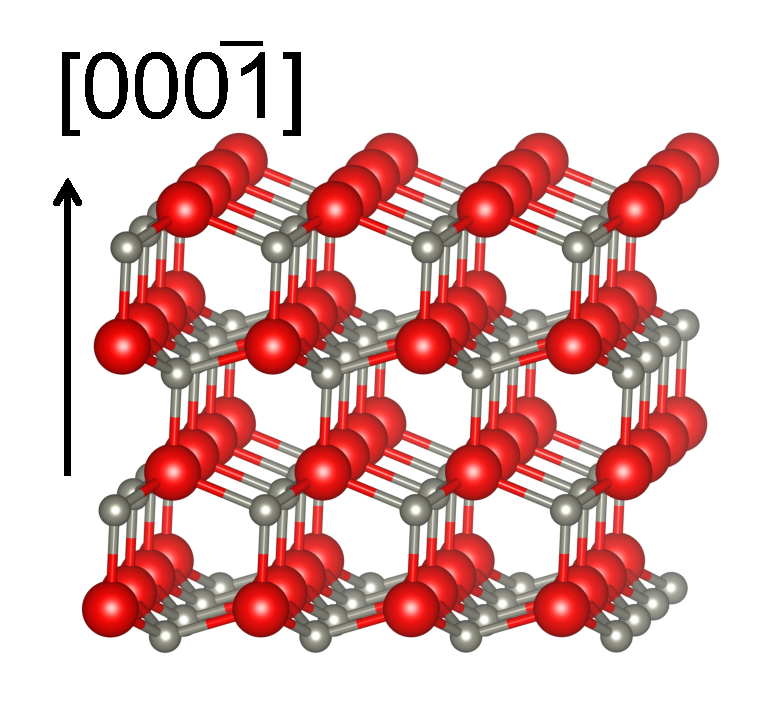
\includegraphics[width=0.47\linewidth]{Chap1/plots/polar1.pdf}}\label{Chap:ZnO_H:fig:ZnO}
  \subfigure[]{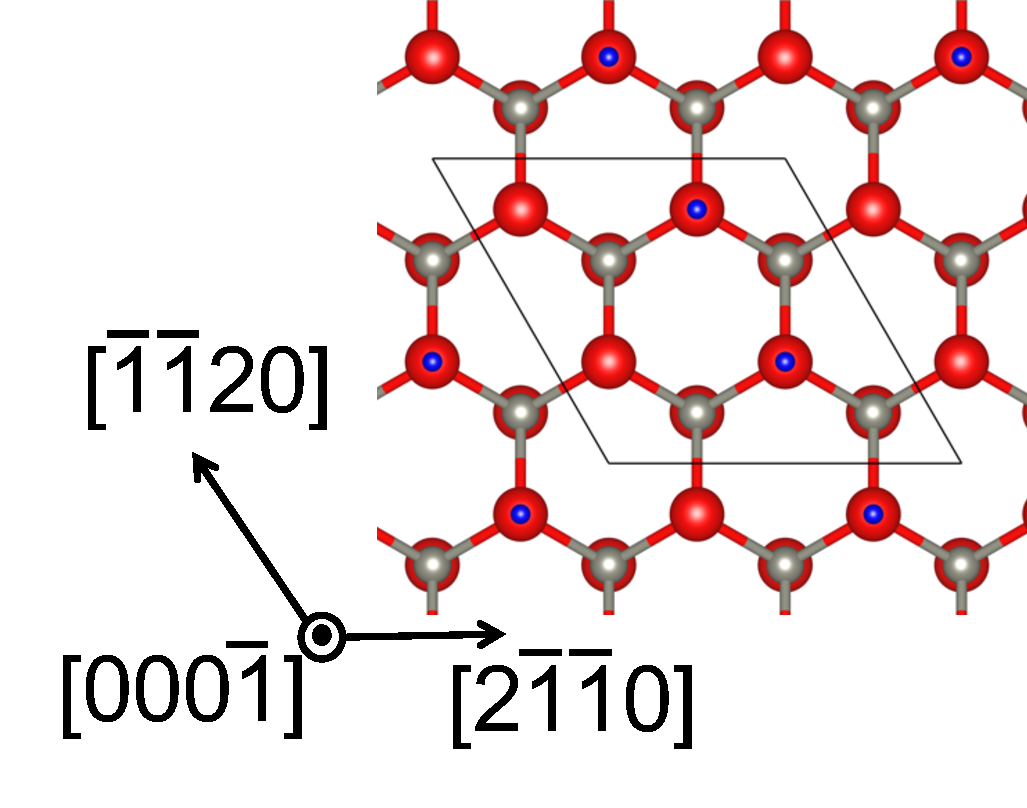
\includegraphics[width=0.47\linewidth]{Chap1/plots/surface2x2.pdf}}\label{Chap:ZnO_H:fig:ZnOSurf}
\caption[Schematic of (2$\times$2) supercell used to model  (000$\bar{1}$) wurtzite ZnO surface with H adsorption.]{(a) and (b): Schematic of (2$\times$2) supercell used to model  (000$\bar{1}$) wurtzite ZnO surface with H adsorption. Large red, small grey and small blue atoms are O, Zn and H atoms, respectively. (a) is the side view projection of ZnO (000$\bar{1}$) slabs, (b) is the top view of (2$\times$2) O-terminated (000$\bar{1}$)  ZnO surface with $\frac{1}{2}$ ML adsorbed H.}
\label{fig1}
\end{figure}
\endgroup

We performed first-principles calculations based on \ac{DFT} by using \ac{VASP} \cite{kresse1996efficient,kresse1999ultrasoft}. Projector augmented wave (PAW) \cite{blochl1994projector} potentials with Perdew-Burke-Ernzerhof (PBE) \cite{perdew1996generalized} exchange-correlation functional and the Hubbard U correction \cite{dudarev1998electron} were used. We applied GGA+U with $U_\text{eff}=U - J = 5.0 eV$ on Zn \textit{d} orbitals as reported in literature\cite{huang2012detailed, oba2010native}. Several other Hubbard U correction parameters ($\text{U}_\text{eff} =$ 3.0 or 7.5 eV) were also tested and showed no significant effects on H adsorption energies. K-points sampling for Brillouin zone integration was performed on a grid of 6$\times$6$\times$1, 6$\times$4$\times$1 with Monkhorst-Pack meshing scheme for (2$\times$2) and (2$\times$3) surface, respectively\cite{monkhorst1976special}. An energy cut-off of 450.0 eV was used in the calculation. The electronic convergence threshold was set as $10^{-4}$ eV. The wurtzite ZnO (000$\overline{1}$) surfaces were constructed by periodic supercell slab models. (2$\times$2) supercells with a vacuum layer of 18 $\angstrom$ in the directions perpendicular to the surfaces were applied as shown in Fig. \ref{Chap:ZnO_H:fig:ZnO} and \ref{Chap:ZnO_H:fig:ZnOSurf}. Each slab contains eight layers of Zn-O repeating units along [0001] direction. Since the ZnO surface slab supercell is not symmetric along [0001] direction, we tested the dipole effects on H adsorption energies and found the dipole effects are minimal if the passivation of the Zn-terminated surface eliminates the artificial electron transfer described as the following. So only the results corresponding no dipole corrections are reported in this study.

As shown in Fig. \ref{Chap:ZnO_H:fig:ZnO}, two types of surfaces are exposed, O-terminated (000$\overline{1}$) surfaces and Zn-terminated  (0001) surfaces, are presented in ZnO slab by its bulk-terminated ideal form. In theoretical modeling, if both sides of a surface slab layer are exposed without modifications, there will be unbalanced electron transfer from Zn-terminated surface to O-terminated surface\cite{Meyer03}. In reality, if the O-terminated surface is exposed to the external environment, the Zn-terminated surface usually is connected to a substrate, which can act as an electron reservoir and compensate unsaturated electrons on the Zn-terminated surface. Many methods have been applied to reduce this artificial electron transfer, such as the introduction of pseudo-hydrogen passivation atoms, Zn vacancies and other adsorbates on Zn-terminated surfaces\cite{calzolari2013dipolar,lin2007microscopic,lahmer2015effect}.

In this work, we focused on O-terminated (000$\overline{1}$) ZnO surface, where H atoms are adsorbed on the top of each surface O atoms as shown in Fig. \ref{Chap:ZnO_H:fig:ZnOSurf}. Zn-terminated (0001) surface on the other side of the slab model was passivated by two different methods to exam their effect on long-distance surface-to-surface electron transfer in the same supercell \cite{zhang2018tuning}. First, $\frac{1}{4}$ ML of Zn vacancy was introduced on the top layer of the Zn-terminated surface in a (2$\times$2) supercell. Second, pseudo-hydrogen atoms with different numbers of valence electrons were introduced on the top layer of the Zn-terminated surface. Each Zn atom on the top layer of the Zn-terminated surface was bonded with one pseudo-hydrogen atom, which can have 1.5, 1.0 or 0.5 electrons (denoted as H$_{1.5}$, H$_{1.0}$ and H$_{0.5}$, respectively). In this paper, all the adsorption energy calculations and electronic structure analyses were conducted on the supercells with H$_{1.5}$-passivated Zn-terminated surfaces unless otherwise specified. The reason will be explained and verified in App. \ref{appd:passivation}.

In this paper, hydrogen adsorption energy $E_{\textup{ad}}^{\textup{H}}$ with H surface coverage $\theta_{\textup{H}}$ equal to $\frac{n}{m}$ ML is calculated as:
\begin{equation}
  \begin{array}{rcl}
       E_{\textup{ad}}^{\textup{H}}(\theta_{\textup{H}}=\frac{n}{m} \textup{ML})&=&E_{\textup{slab+}n\textup{ H}}-E_{\textup{slab+}(n-1) \textup{ H}}-\frac{1}{2}E_{\textup{H}_{2}}
  \end{array}
  \label{eq1}
\end{equation}
Here $E_{\textup{slab+}n \textup{H}}$ and $E_{\textup{slab+}(n-1) \textup{H}}$ is the total energy of surface slab supercell containing $n$ and $n-1$ adsorbed H atoms, respectively, and $E_{\textup{H}_{2}}$ is the energy of an isolated H$_2$ molecule. The ($x\times y$) surface slab supercell itself contains $m=x\cdot y$ duplicates of (1$\times$1) unit cell of 2D surface lattice, so $m=4$ and $m=6$ for (2$\times$2) and (2$\times$3) slab supercells, respectively. As shown in Fig. \ref{Chap:ZnO_H:fig:Ead}, $E_{\textup{ad}}^{\textup{H}}$ on platinum (Pt) (111) surface only increases slightly with a rising surface H coverage $\theta_{\textup{H}}$ ($\delta E_{\textup{ad}}^{\textup{H}}$ $\sim0.1$ eV when  $\theta_{\textup{H}}$ increases from $\frac{1}{4}$ ML to 1 ML ). On the contrary, $E_{\textup{ad}}^{\textup{H}}$ is highly negative and increases slightly on (2$\times$2) slab supercell of (000$\overline{1}$) ZnO when  $\theta_{\textup{H}}$ = $\frac{1}{4}$ and $\frac{1}{2}$ ML, then $E_{\textup{ad}}^{\textup{H}}$ jumps up suddenly after $\theta_{\textup{H}}$ above $\frac{1}{2}$ ML. 

\begingroup
\begin{figure}[!ht]
  \centering
  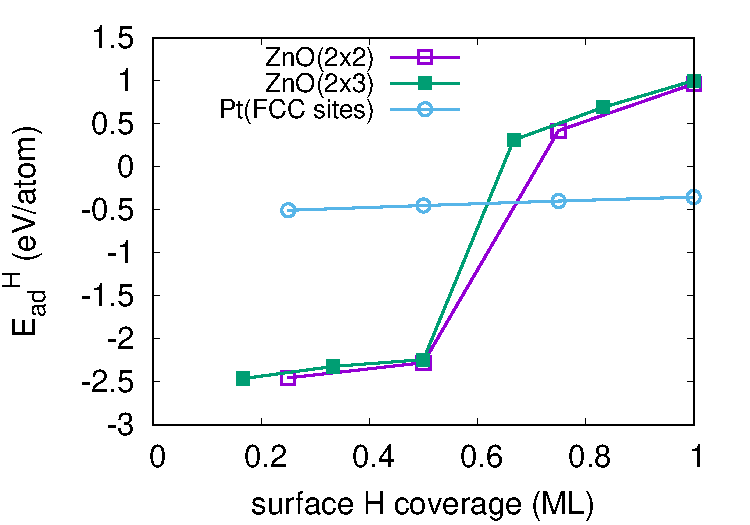
\includegraphics[width=0.9\linewidth]{Chap1/plots/Eadh_coverage_H.pdf}
\caption[H adsorption energies on ZnO surfaces with different H coverage]{H adsorption energies $E_{\textup{ad}}^{\textup{H}}$ defined by Eq. \ref{eq1} on ZnO (000$\overline{1}$) and Pt (111) surfaces with different H coverage}
  \label{Chap:ZnO_H:fig:Ead}
\end{figure}
\endgroup

In order to confirm the critical transition, $E_{\textup{ad}}^{\textup{H}}$ for a larger wurtzite ZnO (000$\overline{1}$) slab supercell with (2$\times$3) in-plane periodicity was also studied. The abrupt increase of $E_{\textup{ad}}^{\textup{H}}$, again, happens when $\theta_{\textup{H}}$ is higher than $\frac{1}{2}$ ML, as shown in Fig. \ref{Chap:ZnO_H:fig:Ead}. It can be concluded that there is a large driving force ($E_{\textup{ad}}^{\textup{H}}$ $<$ -2 eV per H atom) for an isolated H$_2$ molecule to dissociate into two H atoms adsorbed on ZnO (000$\overline{1}$) surface if $\theta_{\textup{H}}$ smaller than $\frac{1}{2}$ ML, above which such adsorption-dissociation reaction becomes highly endothermic and difficult to occur ($E_{\textup{ad}}^{\textup{H}}$ $>$ 0). These results are consistent with previous theoretical calculations and experimental characterizations that $\frac{1}{2}$ ML of adsorbed H were often observed on ZnO (000$\overline{1}$) surface\cite{lin2007density,meyer2004first,lauritsen2011stabilization}.
